\documentclass{article}
\usepackage{graphicx} 
\usepackage{listings}

\begin{document}

\title{TCP File Transfer Protocol}
\author{Tran Minh Anh BI12-015}

\maketitle

\section{Protocol Design}

The protocol follows a basic request-response pattern:

\subsection{Client}

1. Client side source code\newline

\begin{lstlisting}[language=C, caption=Client Code, label=lst:code]
  #include <stdio.h>
  #include <stdlib.h>
  #include <unistd.h>
  #include <string.h>
  #include <arpa/inet.h>
  
  #define SIZE 1024
  
  void send_file(FILE *fp, int sockfd)
  {
      char data[SIZE] = {0};
  
      while(fgets(data, SIZE, fp)!=NULL)
      {
          if(send(sockfd, data, sizeof(data), 0)== -1)
          {
              perror("[-] Error in sending data");
              exit(1);
          }
          bzero(data, SIZE);
      }
  }
  
  int main()
  {
      char *ip = "127.0.0.1";
      int port = 8080;
      int e;
  
      int sockfd;
      struct sockaddr_in server_addr;
      FILE *fp;
      char *filename = "file.txt";
       sockfd = socket(AF_INET, SOCK_STREAM, 0);
      if(sockfd<0)
      {
          perror("[-]Error in socket");
          exit(1);
      }
       printf("[+]Server socket created. \n");
  
       server_addr.sin_family = AF_INET;
       server_addr.sin_port = port;
       server_addr.sin_addr.s_addr = inet_addr(ip);
  
       e = connect(sockfd, (struct sockaddr*)&server_addr, sizeof(server_addr));
       if(e == -1)
       {
           perror("[-]Error in Connecting");
           exit(1);
       }
       printf("[+]Connected to server.\n");
       fp = fopen(filename, "r");
       if(fp == NULL)
       {
           perror("[-]Error in reading file.");
           exit(1);
       }
       send_file(fp,sockfd);
       printf("[+] File data send successfully. \n");
       close(sockfd);
       printf("[+]Disconnected from the server. \n");
       return 0;
  
  }
\end{lstlisting}
2. Working steps\newline
+ Establish connection through designated port.\newline
+ Send data of designated file to the server.\newline 
3. Proof of concept
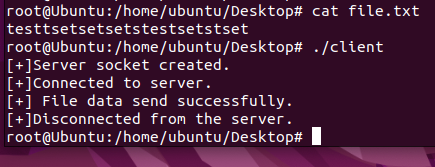
\includegraphics[width=1\linewidth]{client.png}

\subsection{Server}

1. Server side source code\newline 

\begin{lstlisting}[language=C, caption=Server Code, label=lst:code]
  #include <stdio.h>
  #include <stdlib.h>
  #include <string.h>
  #include <arpa/inet.h>
  
  #define SIZE 1024
  
  void write_file(int sockfd)
  {
      int n; 
      FILE *fp;
      char *filename = "file2.txt";
      char buffer[SIZE];
  
      fp = fopen(filename, "w");
      if(fp==NULL)
      {
          perror("[-]Error in creating file.");
          exit(1);
      }
      while(1)
      {
          n = recv(sockfd, buffer, SIZE, 0);
          if(n<=0)
          {
              break;
              return;
          }
          fprintf(fp, "%s", buffer);
          bzero(buffer, SIZE);
      }
      return;
      
  }
  
  int main ()
  {
      char *ip = "127.0.0.1";
      int port = 8080;
      int e;
  
      int sockfd, new_sock;
      struct sockaddr_in server_addr, new_addr;
      socklen_t addr_size;
      char buffer[SIZE];
  
      sockfd = socket(AF_INET, SOCK_STREAM, 0);
      if(sockfd<0)
      {
          perror("[-]Error in socket");
          exit(1);
      }
       printf("[+]Server socket created. \n");
  
       server_addr.sin_family = AF_INET;
       server_addr.sin_port = port;
       server_addr.sin_addr.s_addr = inet_addr(ip);
  
       e = bind(sockfd,(struct sockaddr*)&server_addr, sizeof(server_addr));
       if(e<0)
       {
           perror("[-]Error in Binding");
           exit(1);
       }
       printf("[+]Binding Successfull.\n");
  
       e = listen(sockfd, 10);
       if(e==0)
       {
           printf("[+]Listening...\n");
       }
       else 
       {
           perror("[-]Error in Binding");
           exit(1);
       }
       addr_size = sizeof(new_addr);
       new_sock = accept(sockfd,(struct sockaddr*)&new_addr, &addr_size);
  
       write_file(new_sock);
       printf("[+]Data written in the text file ");
  }
\end{lstlisting}
2. Working steps\newline 
+ Listen for incoming data from specified port.\newline
+ Establish connection once the request is received.\newline 
+ Write received content data in new file.\newline 
3. Proof of concept
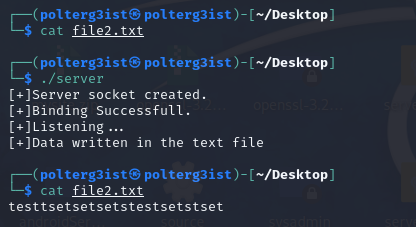
\includegraphics[width=1\linewidth]{server.png}

\end{document}
